\documentclass[aspectratio=169]{beamer}

\usetheme{Boadilla}
\usefonttheme{professionalfonts}
\setbeamertemplate{navigation symbols}{}
\setbeamertemplate{itemize items}[circle]
\setbeamertemplate{enumerate items}[default]
\setbeamertemplate{headline}{}

\usepackage[utf8]{inputenc}
\usepackage[T1]{fontenc}
\usepackage{lmodern}
\usepackage{amsmath}
\usepackage{booktabs}
\usepackage{tabularx}
\usepackage{array}
\usepackage{hyperref}
\usepackage[strings]{underscore}
\usepackage{listings}
\usepackage{tikz}
\usetikzlibrary{arrows.meta,positioning,fit,calc,shapes.geometric}
\usepackage{xcolor}

\definecolor{courseblue}{HTML}{12355B}
\definecolor{coursegold}{HTML}{C98A2E}
\definecolor{courseice}{HTML}{EEF3F8}
\definecolor{coursegreen}{HTML}{2F6B4F}
\definecolor{coursegray}{HTML}{4B5563}
\definecolor{codebg}{HTML}{F7F9FC}
\definecolor{codecomment}{HTML}{5E6C84}
\definecolor{codestring}{HTML}{0B6E4F}

\setbeamercolor{palette primary}{bg=courseblue,fg=white}
\setbeamercolor{palette secondary}{bg=coursegold,fg=white}
\setbeamercolor{palette tertiary}{bg=courseblue,fg=white}
\setbeamercolor{palette quaternary}{bg=coursegold,fg=white}
\setbeamercolor{structure}{fg=courseblue}
\setbeamercolor{frametitle}{bg=courseice,fg=courseblue}
\setbeamercolor{title}{fg=courseblue}
\setbeamercolor{block title}{bg=courseblue,fg=white}
\setbeamercolor{block body}{bg=courseice,fg=black}
\setbeamercolor{normal text}{fg=black,bg=white}
\setbeamercolor{alerted text}{fg=coursegold}

\setbeamerfont{footline}{size=\scriptsize}

\setbeamertemplate{footline}{
  \leavevmode
  \hbox{
    \begin{beamercolorbox}[wd=.33\paperwidth,ht=2.8ex,dp=1.2ex,leftskip=0.8em]{palette primary}%
      University of Trieste
    \end{beamercolorbox}%
    \begin{beamercolorbox}[wd=.49\paperwidth,ht=2.8ex,dp=1.2ex,center]{palette tertiary}%
      \coursename{} \textbar{} \coursecode
    \end{beamercolorbox}%
    \begin{beamercolorbox}[wd=.18\paperwidth,ht=2.8ex,dp=1.2ex,rightskip=0.8em plus1fil]{palette secondary}%
      \insertframenumber{} / \inserttotalframenumber
    \end{beamercolorbox}%
  }
}

\hypersetup{
  colorlinks=true,
  linkcolor=courseblue,
  urlcolor=coursegreen
}

\lstdefinestyle{coursepython}{
  language=Python,
  basicstyle=\ttfamily\footnotesize,
  keywordstyle=\color{courseblue}\bfseries,
  commentstyle=\color{codecomment}\itshape,
  stringstyle=\color{codestring},
  showstringspaces=false,
  columns=fullflexible,
  keepspaces=true,
  frame=single,
  framerule=0.6pt,
  rulecolor=\color{courseblue},
  backgroundcolor=\color{codebg},
  xleftmargin=0.4em,
  xrightmargin=0.4em,
  aboveskip=0.4em,
  belowskip=0.2em
}

\newcommand{\coursename}{Data-driven Systems Engineering}
\newcommand{\coursecode}{440MI / 305SM}
\newcommand{\coursefooter}{}

\newcommand{\learninggoals}[1]{
  \begin{block}{Learning goals}
  #1
  \end{block}
}

\newcommand{\repoactivity}[1]{
  \begin{block}{Repo activity}
  #1
  \end{block}
}

\newcommand{\readinglist}[1]{
  \begin{block}{Papers and materials}
  {\footnotesize #1}
  \end{block}
}

\newcommand{\coursecontextframe}[5]{
  \begin{frame}{Course Map and Running Cases}
  \centering
  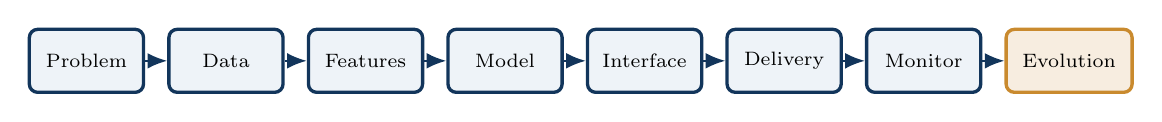
\begin{tikzpicture}[node distance=0.28cm]
  \node[flowbox, minimum width=1.45cm, minimum height=0.8cm] (problem) {\scriptsize Problem};
  \node[flowbox, minimum width=1.45cm, minimum height=0.8cm, right=of problem] (data) {\scriptsize Data};
  \node[flowbox, minimum width=1.45cm, minimum height=0.8cm, right=of data] (features) {\scriptsize Features};
  \node[flowbox, minimum width=1.45cm, minimum height=0.8cm, right=of features] (model) {\scriptsize Model};
  \node[flowbox, minimum width=1.45cm, minimum height=0.8cm, right=of model] (interface) {\scriptsize Interface};
  \node[flowbox, minimum width=1.45cm, minimum height=0.8cm, right=of interface] (delivery) {\scriptsize Delivery};
  \node[flowbox, minimum width=1.45cm, minimum height=0.8cm, right=of delivery] (monitor) {\scriptsize Monitor};
  \node[accentbox, minimum width=1.6cm, minimum height=0.8cm, right=of monitor] (evolution) {\scriptsize Evolution};
  \foreach \a/\b in {problem/data,data/features,features/model,model/interface,interface/delivery,delivery/monitor,monitor/evolution} {
    \draw[arrow] (\a) -- (\b);
  }
  \end{tikzpicture}

  \vspace{0.5em}
  \begin{block}{Today in the course}
  \textbf{Focus:} #1

  \textbf{Bridge:} #2
  \end{block}

  \begin{columns}[T]
  \column{0.48\textwidth}
  \begin{block}{Fraud case}
  {\footnotesize #3}
  \end{block}
  \column{0.48\textwidth}
  \begin{block}{Pasteurization case}
  {\footnotesize #4}
  \end{block}
  \end{columns}

  \vspace{0.3em}
  {\footnotesize \textbf{Course thread:} #5}
  \coursefooter
  \end{frame}
}

\newcommand{\classclosingframe}[4]{
  \begin{frame}{From This Class to the Next}
  \begin{block}{What stays with us}
  #1
  \end{block}

  \begin{columns}[T]
  \column{0.48\textwidth}
  \begin{block}{Project use}
  {\footnotesize #2}
  \end{block}
  \column{0.48\textwidth}
  \begin{block}{Next connection}
  {\footnotesize #3}
  \end{block}
  \end{columns}

  \vspace{0.3em}
  {\footnotesize \textbf{Course thread:} #4}
  \coursefooter
  \end{frame}
}

\tikzset{
  flowbox/.style={
    rounded corners=3pt,
    draw=courseblue,
    fill=courseice,
    very thick,
    minimum width=2.2cm,
    minimum height=0.9cm,
    align=center,
    font=\small
  },
  accentbox/.style={
    rounded corners=3pt,
    draw=coursegold,
    fill=coursegold!15,
    very thick,
    minimum width=2.2cm,
    minimum height=0.9cm,
    align=center,
    font=\small
  },
  arrow/.style={
    -{Latex[length=2.5mm,width=2mm]},
    thick,
    draw=courseblue
  }
}


\title{Class 10: Requirements Engineering for ML Systems}
\author{\coursename}
\date{}

\begin{document}

\frame{\titlepage \coursefooter}

\begin{frame}{Agenda}
\begin{itemize}
\item Introduction, user/system requirements, and quality constraints
\item Functional, non-functional, and domain requirements
\item Specification styles, elicitation, and validation
\item Traceability, change, and requirement management
\item Practice: improving weak ML project requirements
\end{itemize}
\coursefooter
\end{frame}

\begin{frame}{Why requirements are harder for ML systems}
\learninggoals{
\begin{itemize}
\item Distinguish user, system, functional, and non-functional requirements.
\item Write testable requirements instead of vague aspirations.
\item Translate model behavior into system-level acceptance criteria.
\item Connect requirements to later testing, deployment, and monitoring work.
\end{itemize}
}
\coursefooter
\end{frame}

\coursecontextframe
{Requirements that make later validation possible.}
{This class connects stakeholder need to technical behavior so that testing, deployment, and monitoring have something concrete to protect.}
{In the fraud case, requirements include not only prediction quality but latency, logging, explainability, and acceptable false-positive burden.}
{In the pasteurization case, requirements include state visibility, timely alerts, usable thresholds, and operator trust in the dashboard.}
{The course thread here is that weak requirements create confusion that no later engineering step can fully repair.}

\begin{frame}{Why requirements engineering matters so much}
\begin{itemize}
\item Requirements define what success means before implementation begins.
\item Weak requirements create confusion that no amount of modeling skill can repair later.
\item In ML systems, requirements must cover the software, the data, the model behavior, and the operating context.
\end{itemize}
\coursefooter
\end{frame}

\begin{frame}{Types of requirement}
\begin{columns}[T]
\column{0.48\textwidth}
\textbf{User requirements}
\begin{itemize}
\item Natural language
\item Service-level descriptions
\item Written for customers and operators
\end{itemize}
\column{0.48\textwidth}
\textbf{System requirements}
\begin{itemize}
\item Structured and testable
\item Detailed behavior and constraints
\item Used by developers and reviewers
\end{itemize}
\end{columns}
\coursefooter
\end{frame}

\begin{frame}{Why ML systems make requirements harder}
\begin{itemize}
\item Behavior is partly learned from data rather than fully hand-coded.
\item Labels may be delayed, noisy, or disputed.
\item Model performance depends on future data conditions, not only current test data.
\item Stakeholders may ask for ``accuracy'' when they really mean trust, fairness, speed, or interpretability.
\end{itemize}
\coursefooter
\end{frame}

\begin{frame}{Bad requirement vs good requirement}
\begin{block}{Weak}
The fraud system should be fast, accurate, and easy to use.
\end{block}
\begin{block}{Better}
For a batch of 100 review requests, the API shall return a response within 800 ms for at least 95\% of requests, and the review dashboard shall display the top 3 risk indicators used in scoring.
\end{block}
\coursefooter
\end{frame}

\begin{frame}{Functional, non-functional, and domain requirements}
\begin{itemize}
\item Functional: what services the system provides.
\item Non-functional: timing, reliability, security, usability, maintainability.
\item Domain: constraints imposed by the operating environment.
\end{itemize}
\begin{block}{Example}
In pasteurization monitoring, "detect abnormal HeatUp behavior" is functional; "alert within 3 seconds" is non-functional; "respect sensor calibration ranges" is domain-specific.
\end{block}
\coursefooter
\end{frame}

\begin{frame}{Qualities of a good requirement}
\begin{itemize}
\item Necessary: it supports a real stakeholder need.
\item Testable: someone can verify whether it is satisfied.
\item Unambiguous: it is unlikely to be interpreted in different ways.
\item Feasible: it fits known technical and organizational constraints.
\item Traceable: it can be linked to design, tests, and later changes.
\end{itemize}
\coursefooter
\end{frame}

\begin{frame}{Examples tailored to this repository}
\begin{itemize}
\item Functional: the Flask service shall expose `POST /predict` and return JSON.
\item Functional: the pasteurization dashboard shall refresh live sensor plots from the stream endpoint.
\item Non-functional: model inference shall remain deterministic for a fixed artifact and input.
\item Non-functional: drift alerts shall be logged with timestamp and monitored variable.
\end{itemize}
\coursefooter
\end{frame}

\begin{frame}{User stories are not enough by themselves}
\begin{itemize}
\item User stories are helpful for conversation, prioritization, and scope.
\item They still need acceptance criteria to become testable engineering targets.
\item A story without measurable acceptance can hide major ambiguity.
\end{itemize}
\begin{block}{Example}
``As an analyst, I want a fraud score so that I can review risky transactions'' is useful, but it still leaves latency, explanation, threshold logic, and failure behavior unspecified.
\end{block}
\coursefooter
\end{frame}

\begin{frame}{The software requirements document}
\begin{itemize}
\item States what the system should do, not how it should be implemented.
\item Should support communication, traceability, validation, and change control.
\item Varies with context: student prototypes need less detail than regulated industrial systems.
\end{itemize}
\coursefooter
\end{frame}

\begin{frame}{Traceability links requirements to later work}
\begin{itemize}
\item A requirement should connect to design choices, tests, deployment gates, and monitoring rules.
\item Traceability makes change management easier because teams can see what else is affected when one requirement changes.
\item It is especially valuable when the model, pipeline, and interface evolve at different speeds.
\end{itemize}
\coursefooter
\end{frame}

\begin{frame}{Ways to write specifications}
\begin{itemize}
\item Natural language
\item Structured natural language
\item Form-based requirement templates
\item Graphical models such as use cases and sequence diagrams
\item Lightweight formal or tabular specifications when risk is high
\end{itemize}
\coursefooter
\end{frame}

\begin{frame}{Elicitation is structured discovery}
\begin{itemize}
\item Elicitation means discovering requirements from users, operators, policies, data constraints, and business goals.
\item Interviews, observation, document review, and prototype walkthroughs are all useful methods.
\item The purpose is not only to collect wishes, but to reveal conflicts and hidden assumptions.
\end{itemize}
\coursefooter
\end{frame}

\begin{frame}{Good elicitation prompts for project teams}
\begin{itemize}
\item Who acts on the prediction, and what action do they take?
\item What happens if the model is unavailable for one hour?
\item Which inputs may arrive late, missing, or malformed?
\item When do labels appear, and who trusts them?
\item Which requirement is actually a policy or compliance constraint?
\end{itemize}
\coursefooter
\end{frame}

\begin{frame}{Conflicts between requirements are normal}
\begin{itemize}
\item Fast response may conflict with more detailed explanations.
\item High recall may conflict with low false positive rates.
\item Privacy constraints may limit what data can be stored for monitoring or audit.
\item Requirements engineering helps teams make these trade-offs explicit.
\end{itemize}
\coursefooter
\end{frame}

\begin{frame}{Validation techniques that fit student projects}
\begin{itemize}
\item Requirement reviews with a checklist for ambiguity and measurability.
\item Use-case walkthroughs for edge cases and operator behavior.
\item Prototype validation with a minimal dashboard or API client.
\item Acceptance test drafting before full implementation.
\end{itemize}
\coursefooter
\end{frame}

\begin{frame}{Requirements management continues after release}
\begin{itemize}
\item Requirements are not frozen forever because systems, users, and regulations change.
\item Management includes versioning, prioritization, traceability, and impact analysis.
\item In ML systems, drift and changing labels can indirectly trigger new requirements.
\end{itemize}
\coursefooter
\end{frame}

\begin{frame}{Why requirements change}
\begin{itemize}
\item Business priorities shift.
\item New data sources or interfaces appear.
\item Regulations or privacy constraints tighten.
\item Real users expose missing assumptions.
\item The model itself changes what stakeholders ask for.
\end{itemize}
\coursefooter
\end{frame}

\begin{frame}{Requirements connect this course together}
\begin{itemize}
\item Modeling needs evaluation criteria.
\item Delivery pipelines need release checks and acceptance gates.
\item Monitoring needs rules about what deviations matter and who should be informed.
\item MLOps later depends on requirements that were explicit enough to automate.
\end{itemize}
\coursefooter
\end{frame}

\classclosingframe
{\begin{itemize}
\item Requirements make modeling, delivery, and monitoring choices accountable to stakeholder goals.
\item Functional and non-functional expectations are both essential in ML systems.
\item Traceable requirements help teams decide what to build, what to measure, and what to automate.
\end{itemize}}
{A project proposal becomes stronger when it can connect dataset choices, model metrics, interface behavior, and operational checks back to concrete requirements.}
{Class 11 compares process models so teams can decide how to organize work under uncertainty, regulation, and iteration pressure.}
{Explicit expectations make it possible to choose a realistic development process.}

\begin{frame}{Papers and materials}
\readinglist{
\href{https://ieeexplore.ieee.org/document/720574}{IEEE recommended practice for software requirements specifications};\ 
\href{https://www.pearson.com/en-us/subject-catalog/p/software-engineering/P200000003144/9780137035151}{Sommerville, Software Engineering};\ 
\href{https://www.oreilly.com/library/view/practical-mlops/9781098103002/}{Practical MLOps, requirements-to-production perspective};\ 
\href{https://www.altexsoft.com/blog/functional-and-non-functional-requirements-specification-and-types/}{Practical overview of functional and non-functional requirements};\ 
\href{https://www.atlassian.com/agile/project-management/user-stories}{User stories and acceptance criteria guide}.
}
\coursefooter
\end{frame}

\end{document}
